\documentclass[12pt]{article}
\usepackage[utf8]{inputenc}
\usepackage[T2A]{fontenc}
%\usepackage{libertine}
%\usepackage{pscyr}
\usepackage[a4paper, left = 2.5cm,right = 2.5cm,top = 2.5cm,bottom = 3cm]{geometry}
\usepackage[english,russian]{babel}
\usepackage{amsmath}
\usepackage{amssymb}
\usepackage{amsfonts}
\usepackage[final]{graphicx}
\usepackage[linktocpage=true, colorlinks=true, linkcolor = blue, citecolor = red]{hyperref}
\usepackage{cmap}
\usepackage{xfrac}
%\usepackage[titletoc]{appendix}
\usepackage{pgfplots}
\usepackage{cite}
\newcommand{\eprint}{}

%\linespread{1.2}

\newcommand{\bq}{\begin{equation}}
\newcommand{\eq}{\end{equation}}

\usepackage{tikz}

%%%%%%%%%%
\newcommand{\dd}{\partial}
\newcommand{\de}{\delta}
\newcommand{\m}{\mu}
\newcommand{\n}{\nu}
\newcommand{\ls}{\left(}
\newcommand{\rs}{\right)}
\newcommand{\la}{\lambda}
\newcommand{\ka}{\varkappa}
\newcommand{\ga}{\gamma}
\newcommand{\si}{\sigma}
\newcommand{\ta}{\tau}
\newcommand{\al}{\alpha}
\newcommand{\be}{\beta}
\newcommand{\ff}{\varphi}
\newcommand{\te}{\theta}
\newcommand{\sign}{{\rm sign}}
\renewcommand{\sh}{\sinh}
\renewcommand{\ch}{\cosh}

\newcommand{\disn}[2]{$$\displaylines{\refstepcounter{equation}%
            \label{#1}\hskip 1em minus 1em #2\hfilneg}$$}
\newcommand{\nom}{\hfil\hskip 1em minus 1em (\theequation)}
\newcommand{\no}{\hfil \hskip 1em minus 1em\phantom{(\theequation)}%
            \hfilneg\cr\hfilneg\hskip 1em minus 1em\hfil}
\newcommand{\ns}{\hfill\cr\hfill}

%%%%%%%%%%


\begin{document}

\title{Explisit isometric embeddings of collapsing black hole}
\author{
A.~D.~Kapustin\thanks{E-mail: sashakapusta96@gmail.com},
S.~A.~Paston\thanks{E-mail: pastonsergey@gmail.com}\\
{\it Saint Petersburg State University, Saint Petersburg, Russia}
}
\date{\vskip 15mm}
\maketitle

\begin{abstract}
This work is devoted to the search for explicit isometric embeddings of a metric corresponding to the collapse of spherically symmetric matter with the formation of a black hole.
Two approaches are considered, in the first of which an embedding is looked for at once for the whole manifold, and in the second the idea of junction of solutions, obtaining separately for areas inside and outside the dust ball, is used.
In the framework of the first approach, a global smooth embedding in 7D space with a signature (2 + 5) was constructed. It corresponds to the formation of the horizon as a result of matter falling from infinity.
The second approach generally leads to an embedding in 7D space with the signature (1 + 6). This embedding
corresponds to the case when matter flies out of a white hole with the disappearance of its horizon,
after which the radius of the dust ball reaches a maximum, and then a collapse occurs with the formation of the horizon of a black hole.
The embedding obtained is not smooth everywhere --- it contains a break on the edge of the dust ball,
and also not quite global.
In the particular case when the maximum radius of the dust ball coincides with the radius of the horizon, it is possible to construct a global smooth embedding in a flat 6D space with a signature (1 + 5).
\end{abstract}

\clearpage

\section{Introduction}
It is known (see for ex. \cite{goenner}), that an arbitrary (pseudo)Riemannian $d$-dimentional manifold could be \emph{isometrically} embedded in a \emph{flat} ambient space of dimention $N \geqslant d(d+1)/2$ at least locally.
As a result the manifold could be given with the embedding functions $y^a(x^\mu)$, and a metric could be considered as the \emph{induced} one
\bq\label{s1}
	g_{\mu \nu} = (\partial_{\mu} y^a) (\partial_{\nu} y^b) \eta_{ab},
\eq
where $\eta_{ab}$ --- is ambient Minkowski space metric; hereinafter $\mu,\nu=0,...,d-1$; $a,b=1,...,N$.
Such way of manifold description could be visual and useful for its structure study, but it requires finding an explicit expression for the embedding functions of given metric $g_{\mu\nu}$, i.e. one have to solve the differential equation \eqref{s1} w.r.t $y^a$. The manifold structure study are especially actual in case of black holes, because the corresponding manifolds usually have non trivial structure.

The first explicit embedding was constructed in 1921 for the Schwarzschild metrics corresponding to the non-rotating, uncharged black hole \cite{kasner3},
however it (along with the embedding \cite{fudjitani}) is applicable only outside of the horizon, and hence is unsuitable for  studying a structure of the manifold.
The most usefull embedding for such purpose was proposed in 1959 in the work \cite{frons}. It is smooth everywhere
and applicable inside and outside of the horizon, and besides it corresponds to the maximum analytical extension of the Schwarzschild solution,
which includes two areas outside horizon (two universes) and two areas inside horizon, corresponding to a white hole and a black hole.
Beside listed, there is another three so-colled "minimal"{} (i.e. corresponding to the minimal possible dimention
of the ambient space, which in that case is equival to 6 \cite{kasner2}) embeddings \cite{davidson,statja27} of the Schwarzschild metric, which cover a half of the already mentioned maximum analytical extension --- e.g., a set of area outside and area inside, corresponding to black hole,
for details see \cite{statja27}.
It is worth noting, that only this two areas exist, if we considering the Riemannian manifold corresponding to the black hole resulting from the collapse instead of the maximum analytical extension corresponding to the \emph{eternal} black hole.

The problem of finding the minimal \emph{global} (i.e. smooth for any radius value, including horizon points)
embeddings for the non-rotating Reissner-Nordstrom black hole was studied in the work \cite{statja30}.
Three variants of embeddings  was constructed, which could be used in case of a nonextremal charged black hole,
as well as in case of an extremal and the hyperextremal one. A generalization to the case of non zero cosmological constant was studied in the work \cite{statja40}.
In a more interesting from the physical point of view case of the rotating Kerr black hole, as well as in case of its generalization --- the charged rotating Kerr-Newman black hole,
a problem of constructing an explicit embedding becomes much more complicated since that geometries have smaller symetry group.
Only implicitly written (in the form of two differential equations to two unknown components of the embedding function) local embeddings in the 9-dimensional ambient space \cite{kuzeev} and \cite{kuzeevRN} (for the Kerr and Kerr-Newman metric, respectively) and 14-dimensional embedding of the Kerr metric proposed in \cite{gr-qc/0503079} are known.

A constructing explicit embeddings for physically interesting solutions of GR could be usefull
also from the point of the study of the description of gravity in the framework of the embedding theory --- the Regge-Teitelboim gravity, originaly proposed in the work \cite{regge}.
Within the framework of this approach, it is the embedding function $y^a(x)$ that is an independent variable instead of a metric, defined in formula \eqref{s1}.
After \cite{regge} possibility of use an idea of an isometrical embedding for the description of gravity, including in connection with its quantization,
repeatedly discussed in the works of different authors, see for ex.,
works \cite{deser,pavsic85let,tapia,davkar,statja18,rojas09,statja25,faddeev,statja51}.

An explicit embeddings of Riemannian manifolds with horizon are also used in analysis of a connection between Hawking radiation and Unruh radiation, corresponding to the movemnet of the observer in the ambient space \cite{deserlev98,deserlev99,statja34,statja36}.
One can find a detailed list of references, related to the embedding theory and other close issues, in overview \cite{tapiaob}.

A complicity of the problem of constructing explicit embeddings for arbitrary 4-dimentional space-time related to the fact that one have to solve a system of $10$ PDE \eqref{s1} w.r.t embedding functions $y^a(x^\mu)$,
depending on $4$ coordinates $x^\mu$.
The problem is simplified if the manifold has additional symmetries.
The existence of the ones allow us to use constructive method of finding explicit embeddings \cite{statja27}, which could reduce the problem to the solution of the ODE system if the symmetry group is large enough.
This is exactly what happens for the Schwarzschild and Reissner-Nordstrom metrics, with a symmetry group $SO(3)\times T^1$, where $T^1$ denote translational symmetry
corresponding to the shifts of time. A similar situation occcurs (see~\cite{statja29}) in case of cosmological solutions ---
for the metrics of all three FRW models, with symmetries: $SO(4)$ for the closed model, $SO(1,3)$ for the open model
and a group of movements of the three-dimensional plane for the spaеially-flat model.

Probably the most physically interesting variant of a black hole is a black hole resulting from a collapse, when a cloud of matter shrinks and a black hole forms dynamically. In such process a horizon formation occurs
and hence a study of the structure of corresponding manifold becomes very interesting, so the problem of constructing an explicit embedding becomes relevant in that case.
Even if we neglect rotation, i.e. if we will consider that the metric coresponds to Schwarzschild solution in the space around the matter cloud, the problem of constructing an explicit embedding for that metric appears to be very difficult. It is the construction of such embeddings that the present work is devoted to, so far they have not been known.
To simplify the problem, we take the simplest variant of the collapsing matter behavior and consider the collapse of a homogeneous ball consisting of dust-like matter.

The symmetry group of this problem is $SO(3)$, and this symmetry is not large enough to reduce the problem to the solution of the ODE system in the framework of the method \cite{statja27}. However, if we consider a manifold as a set of two parts ---
the first contains matter (compressing or expanding dust ball) and the second doesn't contain it (area outside that ball), then a symmetry group is larger for each part and it can simplify the problem. For an area outside the ball, the metric, according to the well-known Birkhoff theorem, is the Schwarzschild metric. Therefore, it has the symmetry $SO(3) \times T^1$ and we know for it teh set of embeddings mentioned above. For an area inside the ball, the metric coresponds to one of the FRW models, see for ex., \cite{landavshic2},
and hence, it also has an extended symmetry of the corresponding type and the embeddings for this metric are also known \cite{robertson1933}.

This situation allow us to find embeddings for the whole manifold by junction of the modified in appropriate way
known embeddings of its parts. This method is used in the section~4. For the more interesting case of a dynamically forming horizon we have succeed in constructing an embedding in a 7-dimensional ambient space with signature $(+------)$, however it contain a break (discontinuity of the first derivative of the embedding function), and also it cannot be extended to an area of arbitrarily large radii. For the case of the presence of a static horizon, when matter is completely under it, flying out of a white hole and falling into a black hole, a smooth embedding into 6-dimentional ambient space with signature $(+-----)$ is constructed.

An alternative way of constructing such an embedding is an attempt to build it in a uniform way, without using a junction of known embeddings. It is worth noting that in this case a homoginity of a dust ball simplify the problem and allow us to find an explicit embedding for collapse, i.e. for the case of a dynamicaly forming horizon.
This approach is used in section~3.
In this way, it is possible to construct an embedding in a 7-dimensional ambient space with the signature $(+-+----)$, and it turns out to be smooth.




\section{Expression for the metric and used coordinate frames}
We write the expression for the metric that corresponds to a compressing (or expanding) dust ball of finite size. This metric should be a solution to the Einstein equations.
\begin{equation}
\label{G=T}
	G_{\mu \nu} = \varkappa\, T_{\mu \nu}
\end{equation}
with EMT, corresponding to the selected type of matter and it distribution.
The dustlike EMT has the simplest form, if we use a comoving coordinate frame.
Due to spherical symmetry it is convenient to use angles $\theta$ и $\varphi$ as two spatial coordinates.
Remaining timelike coordinate we denote as $\tau$, and spatial one as -- $\chi$.

The described solution of the Einstein equations can be found in the form of a diagonal metric. For the arbitrary destribution of matter w.r.t. radius a corresponding squared interval (further we will refer to such formulas as metric) has form \cite{landavshic2}
\bq
\label{metric}
	d s^2 = d \tau^2 - \frac{(r'(\tau, \chi))^2}{1+f(\chi)} d\chi^2 - r^2(\tau, \chi) d \Omega^2,
\eq
where $d\Omega^2=d\theta^2+sin^2\theta d\varphi^2$, and
function $r(\tau, \chi)$ is determined by one of three ways
\bq
\label{v123}
	r(\tau, \chi) = \left\{
	\begin{array}{l}
	\vphantom{\Biggr(}
    \dfrac{F(\chi)}{2 f(\chi)} H \left( \dfrac{2(f(\chi))^{\sfrac{3}{2}} }{F(\chi)}(\tau_0(\chi)-\tau)  \right) , \ \ \ \ f(\chi) > 0,\\
	\left( \dfrac{9F(\chi)}{4} \right)^{\sfrac{1}{3}} \left[ \tau_0(\chi)- \tau \right]^{\sfrac{2}{3}}, \ \ \ \ f(\chi) = 0, \\
	- \dfrac{F(\chi)}{2 f(\chi)} E \left( \dfrac{2(-f(\chi))^{\sfrac{3}{2}} }{F(\chi)}(\tau_0(\chi)-\tau) \right), \ \ \ \ f(\chi) < 0.
	\end{array} \right.
\eq
Functions $H(x)$ and $E(x)$ is used for inversion of parametric dependencies
\bq\label{sp4}
H = \ch{\eta}-1,\quad x = \sh{\eta} - \eta;\qquad
E = 1 - \cos{\eta},\quad x = \eta - \sin{\eta},
%	\begin{array}{c}
%	E = 1 - \cos{\eta}, \\
%	x = \eta - \sin{\eta},
%	\end{array} \ \ \ \ \ \ \ \
%	\begin{array}{c}
%	H = \ch{\eta}-1, \\
%	x = \sh{\eta} - \eta,
%	\end{array}
\eq
and functions $F(\chi), f(\chi)$ and $\tau_0(\chi)$ define a matter density distribution and it's initial speed.
In this case, the function $F(\chi)$ has the meaning of the Schwarzschild radius of all matter having a coordinate value less than $\chi$, and the function $\tau_0 (\chi)$ determines the time instant $\tau$ at which the particle with coordinate $\chi$ reaches the point $r = 0$, i.e. will fall on the singularity resulting from the collapse.

If we require a homogenious distribution of matter at the initial moment, then the space inside the collapsing ball will be described by the geometry of the open, spatially flat or closed FRW model, respectively, by choosing the first, second or third method of determining $ r(\tau, \chi)$ in the formula \eqref{v123}.
It is easy to notice that the homogeneity at each moment of time requires the simultaneity of the fall of all particles to the point $r = 0$, as a result of which the function $\tau_0(\chi)$ should turn into a constant and it can be taken equal to zero by choosing the time $\tau$.

The outer space to the ball, according to the Birkhoff theorem, in all cases is described by the Schwarzschild geometry.
Since the matter density is equal to zero in this area, the total mass of matter having a coordinate value less than given $\chi$ are no longer depend on $\chi$. Therefore, the Schwarzschild radius of this matter is constant, and therefore the substitution of $ F (\ chi) = const $ into the formula (\ ref {metric}) corresponds to the obtaining of the Schwarzschild metric.

If a matter density inside the ball is constant, and hence, has a jump on the boundary of the ball, then the metric (\ref{metric}) will have a coordinate peculiarity in the form of a jump on the boundary of the ball, which can be excluded by the change of the coordinate frame to the $(\tau, r, \theta, \varphi)$.
If we make such a change of coordinates, then the metric \eqref{metric} takes the form
\bq\label{sp1}
	d s^2 = \left( 1- \frac{\dot{r}(\tau, \chi)^2}{1+f(\chi)}\right) d \tau^2 + 2\frac{\dot{r}(\tau, \chi)}{1+f(\chi)}dr d\tau - \frac{dr^2}{1+f(\chi)} - r^2 d\Omega^2,
\eq
where $\dot{r}(\tau, \chi) \equiv \frac{\partial r(\tau, \chi)}{\partial \tau}$, and $r(\tau, \chi)$ is given by \eqref{v123}.
The value $\chi$ entering into \eqref{sp1} through $\dot{r}(\tau, \chi)$ and $f(\chi) $ must be expressed in terms of the independent coordinates $ \tau $ and $ r $ according to \eqref{v123}.

Then if we choose in \eqref{v123} a variant $f(\chi)=0$, then the situation will become much simpler, because $r(\tau, \chi)$ and $\dot{r}(\tau, \chi)$ can be written explicitly. After simple transformations, the metric will take the form
\bq
\label{metric2}
	d s^2 = \left(1-\frac{F(\tau, r)}{r} \right)d\tau^2 - 2 \sqrt{\frac{F(\tau, r)}{r}}dr d\tau  - dr^2 - r^2 d\Omega^2,
\eq
where hereinafter $F(\tau, r)\equiv F(\chi(\tau, r))$.
While the matter density remain finite, this metric, written in the coordinates $(\tau, r, \theta, \varphi)$, will be continuous due to the continuity of the function $F(\chi)$ in this case.

Inside of the homogeneous dust ball we can assume $\tau_0(\chi)=0$ (see after the formula \eqref{sp4}), which makes it easy to find in this area the expression for function $F(\tau, r)$ from \eqref{v123}, in case $f(\chi)=0$. Considering that outside the ball $F(\chi) = const$ and assuming continuity of $F(\chi)$, in general, one can find
\bq\label{sp2}
	F(\tau, r) = \min{ \left( \frac{4r^3}{9\tau^2}, F_0 \right) },
\eq
where $F(\tau, r)=F_0$ outside of the ball. Here, we assume that the time $ \ tau $ is everywhere negative and changes to its zero value, which corresponds to the end of the collapse, when the whole matter simultaneously reached the point $r=0$ and formed the singularity.

The expression for the metric \eqref{metric2} in coordinates $(\tau, r, \theta, \varphi)$ will be used when searching for an explicit embedding in section~3.
The possibility to write the metric in the form \eqref{metric} in synchronous and comoving coordinate frame will be used in section~4.


\section{Constructing the embedding without using a junction of solutions}
We will construct the first variant of an explicit embedding for metric (\ref{metric2}) without using the possibility of joining separate embeddings for the inside and outside of the ball.
In this case, however, we will assume that the dust ball is homogeneous at each moment of time and the formula \eqref{sp2} can be used, since in this case the problem is simplified.
Recall that the value of $F(\tau, r)$ given by this formula, up to a factor, gives the mass of dust contained within the radius $r$ at the time $\tau$. It is easy to notice that according to \eqref{sp2} the metric (\ref{metric2}) is continuous, however its first derivative has a jump on the boundary of the ball.

\begin{figure}[h!]
	\centering
	\begin{tikzpicture}[scale=0.75]
		\draw[->] (-5, 0) -- (5, 0)node[below]{$u$};
		\draw[->] (0, -5) -- (0, 5)node[left]{$v$};
		%%
		\draw[->] (4.5, 0.5) -- (5.5, 0.5)node[midway,above]{$r \to \infty$};
		%%
		\begin{scope}
		\clip (7.5, 6) -- (5, 6) -- (0.6, 2.8) .. controls (1, 1) and (1, 0) .. (5, -3) -- (5, -6) -- (7.5, -6) -- cycle;
		\draw[thick, dashed] (-5, -5) -- (5, 5)node[above right]{$r = R$};
		\draw[thick, dashed] (-5, 5) -- (5, -5);
		%%
		\draw (5, 4.9) .. controls (0, 0) and (0, -0) .. (5, -4.9);
		\draw (5, 4.7) .. controls (1.5, 1) and (1.5, -1) .. (5, -4.7);
		\draw (5, 4.5)node[below right]{$r=const$} .. controls (3, 1.5) and (3, -1.5) .. (5, -4.5);
		%%
		\draw (-5, 4.9) .. controls (0, 0) and (0, -0) .. (-5, -4.9);
		\draw (-5, 4.7) .. controls (-1.5, 1) and (-1.5, -1) .. (-5, -4.7);
		\draw (-5, 4.5) .. controls (-3, 1.5) and (-3, -1.5) .. (-5, -4.5);
		%%
		\draw (4.9, 5) .. controls (0, 0) and (0, 0) .. (-4.9, 5);
		\draw (4.8, 5) .. controls (1, 1) and (-1, 1) .. (-4.8, 5);
		\draw[ultra thick] (4.7, 5) .. controls (2, 2) and (-2, 2) .. (-4.7, 5);
		%%
		\draw (4.9, -5) .. controls (0, 0) and (0, 0) .. (-4.9, -5);
		\draw (4.8, -5) .. controls (1, -1) and (-1, -1) .. (-4.8, -5);
		\draw[ultra thick] (4.7, -5) .. controls (2, -2) and (-2, -2) .. (-4.7, -5);
		\draw (0, -3)node[below right]{$r = 0$};
		%%
		\end{scope}
		\draw (0, 3)node[above right]{$r = 0$};
		\draw[blue, very thick] (5, -3) .. controls (1, 0) and (1, 1) .. (0.6, 2.8);
	\end{tikzpicture}
	\caption{\label{infkrusk}The Kruskal diagram for the matter collapsing from infinity.}
\end{figure}
The area outside of the ball, describing by the Schwarzschild metric, is shown on the Kruskal diagram in Fig.~\ref{infkrusk}.

It is limited by the world line of the point corresponding to the boundary of the ball.
The remaining part of the manifold, corresponding to the interior of the ball, is described by the FRW metric and is not shown in the figure. Since we take $f(\chi)=0$ when moving  from (\ref{metric}) to (\ref{metric2}), this is a metric of the spatially flat model FRW (see \eqref{v123} and text after).

It can be seen from \eqref {sp2}, that the boundary of the ball is described by the equation 
\disn{sp3}{
r^3=\frac{9}{4}F_0\tau^2,
\nom}
from which we can conclude that $r\to\infty$ when $\ta\to-\infty$,
i.e. the size of the dust ball was infinite in the past.
It means that the embedding, constructing in this section, corresponds to collapse of particles, falling from the spacial infinity. Note that this situation is qualitatively different from that considered in section~4.


We will look for the embedding function $y^a(x^\mu)$ in the form of a set of components $\{\tilde y^A(\tau,r),$ $\hat y^i(r,\te,\ff)\}$, where three components $\hat y^i(r,\te,\ff)$ have a usual form for the spherically symmetric embeddings\begin{align}\label{sp7}
\hat y^1 &= r \cos{\theta}, \nonumber\\
\hat y^2 &= r \sin{\theta} \cos{\varphi},  \\
\hat y^3 &= r \sin{\theta} \sin{\varphi}.\nonumber
\end{align}
Then, taking into account the structure of the formula of the induced metric \eqref{s1}, the problem of constructing an explicit embedding for the metric (\ref{metric2}) is reducing to the problem of finding an embedding for a 2-dimentional surface
$\tilde y^A(\tau,r)$ with the metric
\disn{sp8}{
d s^2 = \left(1-\frac{F(\tau, r)}{r} \right)d\tau^2 - 2 \sqrt{\frac{F(\tau, r)}{r}}dr d\tau.
\nom}
To simplify this search, we introduce new variables $t = \tau^{\sfrac{2}{3}}$ and $p = r^3/\tau^2$ instead of $\tau$ and $r$, so \eqref{sp2} will have the form
\bq\label{sp6}
F(\tau, r) = \min{ \left( \frac{4}{9}p, F_0 \right) }\equiv\bar F(p).
\eq
Then we can obtain a following expression fo th emetric (\ref{sp8})
\bq\label{eq10}
	d s^2 = \left(\frac{9}{4} t +f(p) \right) dt^2 + t\, p^{-\sfrac{5}{6}}\sqrt{\bar F(p)} \, dp\, dt,
\eq
where
\bq\label{eq10.1}
f(p) = 3 p^{\sfrac{1}{6}} \sqrt{\bar F(p)}-\frac{9}{4}p^{-\sfrac{1}{3}} \bar F(p).
\eq

The components of the metric (\ref{eq10}) are a polinomials with respect to the variable $t$. It allow us to look for the corresponding components of the embedding functions $\tilde y^A(t,p)$ also in the form of polinomials of $t$, in the way, similar to the one used in the work\cite{statja27} for constructing the "cubic"{} embedding of the Schwarzschild metric. The embedding was found for the case of 4-dimentional ambient space with the signature $(+-+-)$. Using the light-like coordinates in the ambient space $\tilde y^\pm=\tilde y^0\pm\tilde y^1$, it can be written in the form
\begin{align}\label{sp9}
	\tilde y^{+} &= 2t^3 + \frac{9}{8}t^2+tf(p), \nonumber\\
	\tilde y^2 &=  w(p), \\
	\tilde y^{-} &= t, \nonumber\\
	\tilde y^{3} &= \sqrt{\frac{3}{2}}t^2 -w(p)\nonumber,
\end{align}
где
\disn{sp9.1}{
w(p)=\frac{1}{2\sqrt{6}}\ls\int\!\sqrt{\bar F(p)}\,p^{-\sfrac{5}{6}} dp- f(p)\rs=\ns=
\frac{1}{\sqrt{6}}\te\ls p-\frac{9}{4}F_0\rs
\ls\ls\frac{9}{4}F_0\rs^{\sfrac{1}{2}}p^{\sfrac{1}{6}}+\frac{9}{8}F_0p^{-\sfrac{1}{6}}-\frac{3}{2}\ls\frac{9}{4}F_0\rs^{\sfrac{2}{3}}\rs
\nom}
и $\te(z)$ -- тэта-функция Хевисайда (при вычислении \eqref{sp9.1} использован явный вид \eqref{sp6} функции $\bar F(p)$).

Возвращаясь к более естественным координатам $\tau$, $r$ и объединяя компоненты \eqref{sp9}
с оставшимися компонентами \eqref{sp7} полной функции вложения $y^a(x^\mu)$,
окончательно получаем функцию вложения для метрики (\ref{metric2}) в виде
\begin{align}\label{sp10}
	y^0 &= \tau^2 + \frac{9}{16}\tau^{\sfrac{4}{3}}+\frac{1}{2}\tau^{\sfrac{2}{3}} \ls f\ls\frac{r^3}{\tau^2}\rs+1\rs, \nonumber\\
	y^1 &= \tau^2 + \frac{9}{16}\tau^{\sfrac{4}{3}}+\frac{1}{2}\tau^{\sfrac{2}{3}} \ls f\ls\frac{r^3}{\tau^2}\rs-1\rs, \nonumber\\
	y^2 &=  w\ls\frac{r^3}{\tau^2}\rs, \\
	y^3 &= \sqrt{\frac{3}{2}}\tau^{\sfrac{4}{3}}-w\ls\frac{r^3}{\tau^2}\rs, \nonumber\\
	y^4 &= r \cos{\theta}, \nonumber\\
	y^5 &= r \sin{\theta} \cos{\varphi},  \nonumber\\
	y^6 &= r \sin{\theta} \sin{\varphi},\nonumber
\end{align}
причем объемлющее пространство 7-мерно и обладает сигнатурой $(+-+----)$.
Напомним, что время $\tau$ предполагается всегда отрицательным, а его нулевое значение
соответствует падению всех частиц пылевого шара в точку $r=0$.

Построенное вложение является глобальным в том смысле, что оно остается гладким при всех значениях $r$
и всех $\tau<0$, т.е. до момента образования сингулярности.
Исследуем степень имеющейся гладкости при $\tau<0$.
Прежде всего, при использовании сферических координат нужно проверить отсутствие нарушения гладкости
в точке $r=0$. Для этого достаточно проверить, что компоненты $y^0$,$y^1$,$y^2$,$y^3$ в этой точке конечны и не имеют в ней
нечетных степеней разложении по $r$. Поскольку при $p<9F_0/4$ оказывается $f(p)=p^{\sfrac{2}{3}}$, $w(p)=0$
(см. \eqref{sp6},\eqref{eq10.1},\eqref{sp9.1}), то это оказывается именно так.
Далее, нужно проверить степень гладкости на границе пылевого шара, что соответствует значению аргумента $p=9F_0/4$
функций $f(p)$, $w(p)$.
Как показывает простой анализ тех же формул, в указанной точке функции $f(p)$ и $w(p)$ непрерывны вместе со своими первыми производными,
но их вторые производные испытывают скачок. Графики этих функций при $F_0=1$ приведены на рис.~\ref{graf-f-w}.
\begin{figure}[h!]
\centering
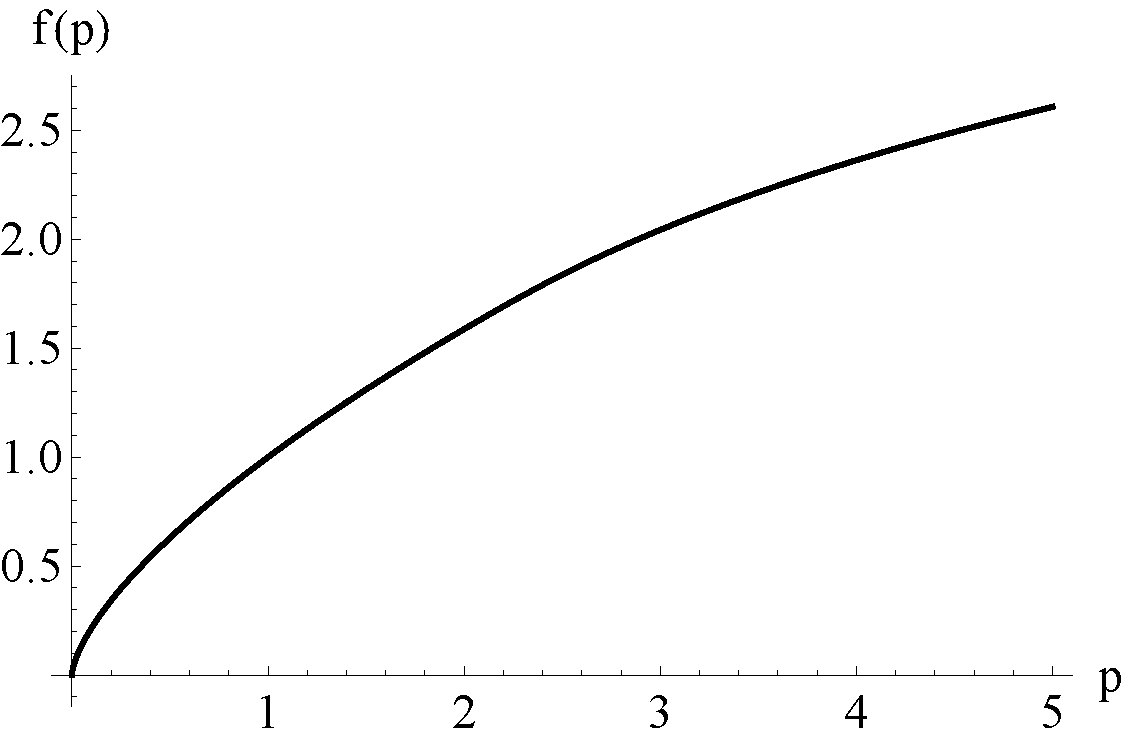
\includegraphics[width=0.45\linewidth]{graf_f.pdf}
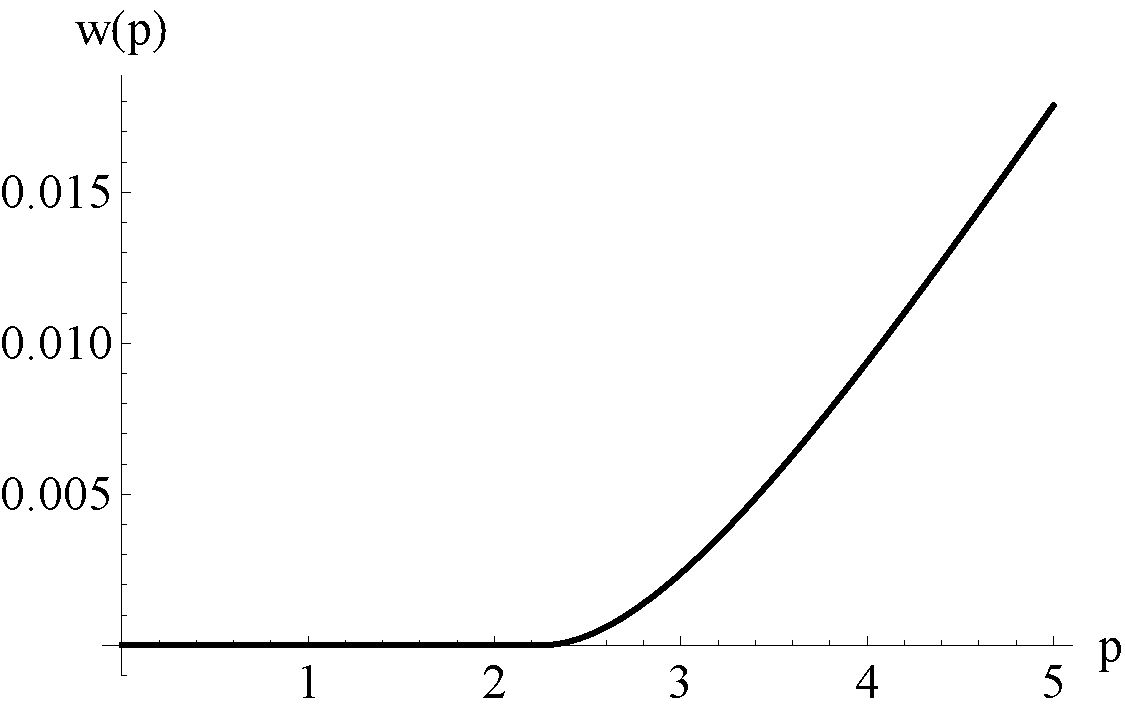
\includegraphics[width=0.45\linewidth]{graf_w.pdf}
\caption{\label{graf-f-w}
Графики функций $f(p)$ и $w(p)$ при $F_0=1$.
}
\end{figure}

Таким образом, построенная явная функция вложения \eqref{sp10} является непрерывно дифференцируемой.
Разрыв ее вторых производных соответствует скачку плотности материи на границе пылевого шара, так что гладкость вложения
соответствует физической постановке задачи. Проекция двумерной поверхности, соответствующей \eqref{sp10}
при фиксированных углах $\theta,\varphi$, на трехмерное подпространство $y^0,y^3,y^4$ изображена
на рис.~\ref{pic_emb1}.
\begin{figure}[h!]
\centering
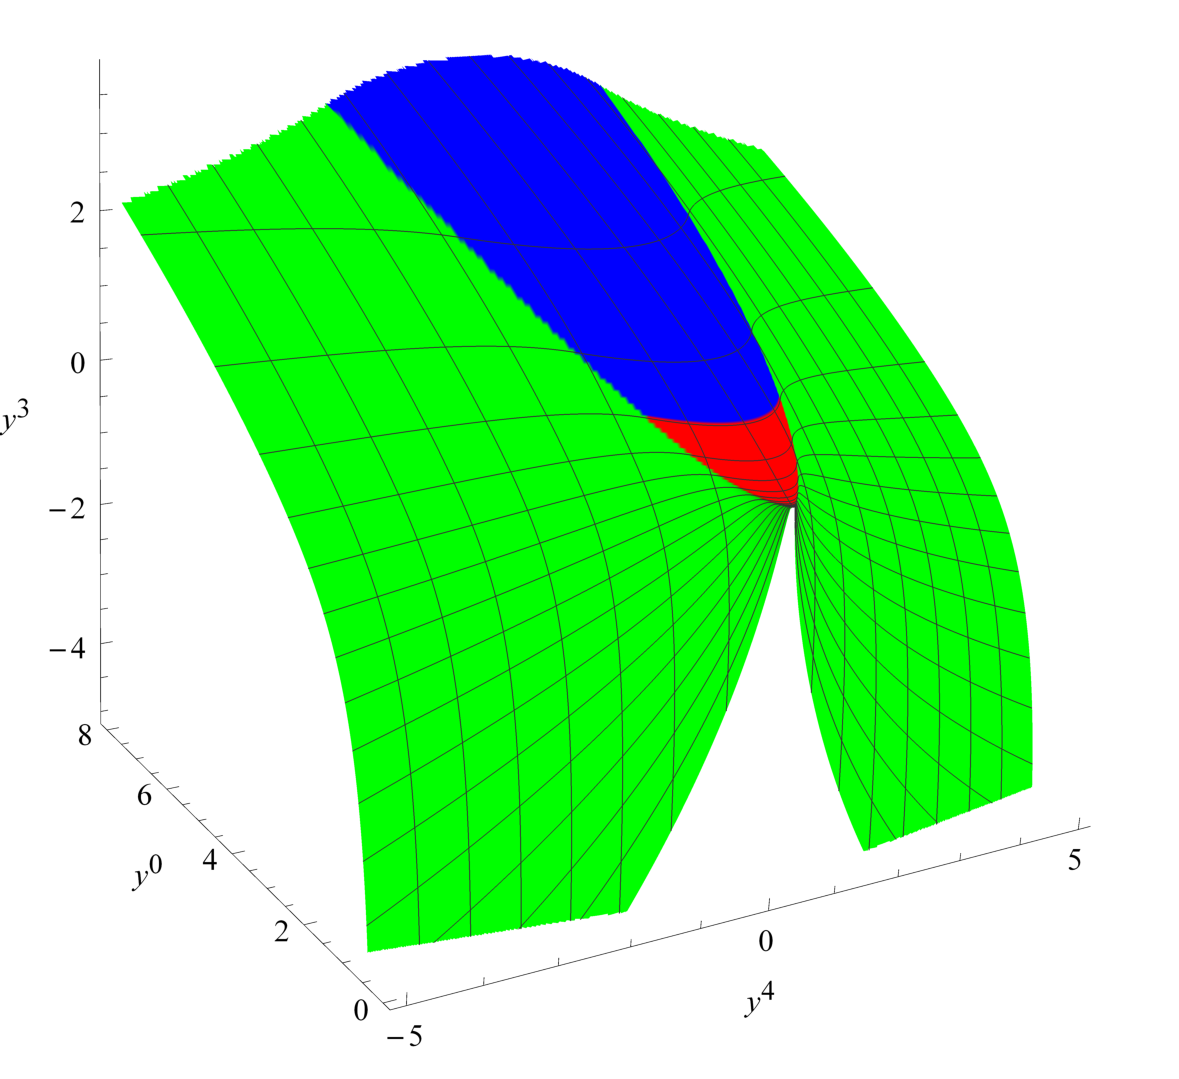
\includegraphics[width=0.55\linewidth]{col_emb-c2.pdf}
\caption{\label{pic_emb1}
Проекция двумерного подмногообразия $\theta,\varphi=const$ вложения \eqref{sp10} на подпространство $y^0,y^3,y^4$.
}
\end{figure}
Зеленым показана область вне пылевого шара, синим и красным -- область пыли до и после образования горизонта, соответственно.
Возникающей в результате коллапса сингулярности соответствует значение $y^0=0$. Интересно отметить, что
в окрестности этой области вид поверхности оказывается сходным с поведением вблизи сингулярности
вложения \cite{robertson1933} для пространственно-плоской модели FRW.

Найденный в этом разделе вариант вложения использует объемлющее пространство с двумя времениподобными направлениями,
что можно считать его недостатком с точки зрения попыток придать объемлющему пространству физический смысл.
В следующем разделе мы пытаемся устранить этот недостаток, используя еще один способ построения явного вида вложения,
основанный на сшивке вложений двух частей пространства-времени, соответствующих областям внутри и вне пылевого шара.


\section{Построение вложения с помощью сшивки}
Будем искать вложение для метрики \eqref{metric}, записанной в сопутствующей системе координат, несмотря на то, что
в этих координатах метрика содержит координатную особенность (см. перед формулой \eqref{sp1}).
Мы воспользуемся известными вложениями для областей внутри (метрика FRW) и вне  (метрика Шварцшильда)
пылевого шара, модифицировав их таким образом, чтобы полученные функции вложения можно было сшить.

В сопутствующих координатах уравнение движения материи имеет вид $\chi = const$, поэтому можно сказать, что область $0 \leqslant \chi < \chi_0$ содержит материю, область $\chi > \chi_0$ соответствует пустому пространству, а $\chi = \chi_0$ --- граница пылевидного шара.
Выберем $r(\tau, \chi)$ в формуле (\ref{v123}) согласно третьему способу, что соответствует закрытой модели FRW в случае однородной плотности материи.
Тогда при выборе функций
\bq
F(\chi) = \frac{R \sin^3{\chi}}{\sin^3{\chi_0}}, \qquad f(\chi) = -\sin^2{\chi}, \qquad \tau_0(\chi) = const,
\eq
отвечающем постоянной плотности пыли, при $0 \leqslant \chi < \chi_0$, выражение для $r(\tau, \chi)$ примет вид
\bq\label{sp14}
	r(\tau, \chi) = \frac{R \sin{\chi}}{2 \sin^3{\chi_0}}  E \left( \pi - \frac{2 \sin^3{\chi_0}}{R} \tau \right).
\eq
Здесь $R$ -- радиус Шварцшильда всего пылевого шара, определяемый его полной массой, а
параметр $\chi_0$ определяет максимальный размер шара $r_{max} = R/\sin^2{\chi_0}$,
так как определяемая \eqref{sp4} функция $E(x)$ принимает значения от $0$ до $2$.
Значение $\tau_0$ выбирается так, чтобы момент $\tau = 0$ соответствовал максимальному размеру шара.
При этом время $\tau$ изменяется в конечных пределах $\tau\in [-\pi R/(2\sin^3{\chi_0}),\pi R/(2\sin^3{\chi_0})]$,
причем начальное и конечное значения соответствуют выходу материи из сингулярности в прошлом и ее падению в сингулярность в будущем.

Подстановка функции $r(\tau, \chi)$ в таком виде в формулу (\ref{metric}) дает метрику FRW
\bq\label{sp19}
ds^2 = d\tau^2 - a^2(\tau) \left(d\chi^2 + \sin^2{\chi}d\Omega^2 \right)
\eq
с масштабным параметром вида
\bq\label{spp1}
a(\tau) = \frac{R}{2 \sin^3{\chi_0}} E \left( \pi - \frac{2 \sin^3{\chi_0}}{R} \tau \right).
\eq

При $\chi > \chi_0$ можно выбрать
\bq\label{spp1a}
r(\tau, \chi) = \frac{r_m(\chi)}{2} E \left( \pi - \frac{2R^{\sfrac{1}{2}}}{r^{\sfrac{3}{2}}_m(\chi)} \tau \right),
% \ \ \ \ \text{при } ,
\eq
что соответствует метрике Шварцшильда (см. \cite{landavshic2,novfrol}).
От присутстующей здесь функции $r_m(\chi)$ требуется только, чтобы она монотонно возрастала
от значения $R/\sin^2{\chi_0}$ при $\chi=\chi_0$ до бесконечности при при $\chi \to \infty$,
а в остальном она может быть выбрана произвольным образом.
%содержит произвол, ограничивающийся лишь требованием непрерывности $r(\tau, \chi)$ и стремлением $r_m \to \infty$ при $\chi \to \infty$.


Область $\chi > \chi_0$
%также может быть
представлена на диаграмме Крускала, приведеной на Рис. \ref{closedkrusk}. По ней видно, что в этом случае крайняя и все внутренние частицы материи вылетают из бело-дырной сингулярности, достигают максимального удаления и коллапсируют в черно-дырную сингулярность. Остальная часть многообразия описывается геометрией FRW, как и в предыдущем случае.
\begin{figure}[h!]
	\centering
		\begin{tikzpicture}[scale=0.75]
			\draw[->] (-5, 0) -- (5, 0)node[below]{$u$};
			\draw[->] (0, -5) -- (0, 5)node[left]{$v$};
			%%
			\draw[->] (4.5, 0.5) -- (5.5, 0.5)node[midway,above]{$r \to \infty$};
			%%
			\begin{scope}
			\clip (7.5, 6) -- (5, 6) -- (0, 3.5) .. controls (0, 1) and (1, 0.5) .. (1, 0) -- (1, 0) .. controls (1, -0.5) and (0, -1) .. (0, -3.5) -- (5, -6) -- (7.5, -6) -- cycle;
			\draw[thick, dashed] (-5, -5) -- (5, 5)node[above right]{$r = R$};
			\draw[thick, dashed] (-5, 5) -- (5, -5);
			%%
			\draw (5, 4.9) .. controls (0, 0) and (0, -0) .. (5, -4.9);
			\draw (5, 4.7) .. controls (1.5, 1) and (1.5, -1) .. (5, -4.7);
			\draw (5, 4.5) .. controls (3, 1.5) and (3, -1.5) .. (5, -4.5)node[above right]{$r=const$};
			%%
			\draw (-5, 4.9) .. controls (0, 0) and (0, -0) .. (-5, -4.9);
			\draw (-5, 4.7) .. controls (-1.5, 1) and (-1.5, -1) .. (-5, -4.7);
			\draw (-5, 4.5) .. controls (-3, 1.5) and (-3, -1.5) .. (-5, -4.5);
			%%
			\draw (4.9, 5) .. controls (0, 0) and (0, 0) .. (-4.9, 5);
			\draw (4.8, 5) .. controls (1, 1) and (-1, 1) .. (-4.8, 5);
			\draw[ultra thick] (4.7, 5) .. controls (2, 2) and (-2, 2) .. (-4.7, 5);
			\draw (0, 3)node[above right]{$r = 0$};
			%%
			\draw (4.9, -5) .. controls (0, 0) and (0, 0) .. (-4.9, -5);
			\draw (4.8, -5) .. controls (1, -1) and (-1, -1) .. (-4.8, -5);
			\draw[ultra thick] (4.7, -5) .. controls (2, -2) and (-2, -2) .. (-4.7, -5);
			\draw (0, -3)node[below right]{$r = 0$};
			%%
		%	\draw[blue, thick] (5, -3)node[above right]{$r_m(t)$} .. controls (1, 0) and (1, 1) .. (0.6, 2.8);
			\end{scope}
			\draw[very thick, blue] (0.03, 2.77) .. controls (0.1, 1) and (1, 0.5) .. (1, 0) -- (1, 0) .. controls (1, -0.5) and (0.1, -1) .. (0.03, -2.77);
		\end{tikzpicture}
	\caption{\label{closedkrusk}The Kruskal diagram for the collapse of matter, which flew out of the white hole singularity.}
\end{figure}

\subsection{Общий случай}      %Построение вложения в общем случае
Согласно \cite{kasner2}, минимальная размерность вложения для метрики Шварцшильда равна~$6$, поэтому известные пятимерные вложения для метрики FRW
% (можно найти в \cite{statja29} или
\cite{robertson1933,rosen65} следует модифицировать добавлением дополнительных функций вложения. Основная идея заключается в том, чтобы <<не трогать>> зависимость функций вложения от координаты $\chi$, а добавить только функции, зависящие от $\tau$. В таком подходе условие выполнения уравнений вложения \eqref{s1} сводится к решению ОДУ относительно добавляемых функций вложения.

Отсюда и далее будем обозначать $y^a_f$ функции, относящиеся к вложению метрики FRW, а $y^a_s$ --- метрики Шварцшильда.
Пятимерное вложение метрики закрытой модели FRW имеет вид
\begin{align}
\label{sp13}	y^0_f &= h(\tau), \\
\label{0}	y^1_f &= a(\tau) \cos{\chi}, \\
\label{1}	y^2_f &= a(\tau) \sin{\chi} \cos{\theta}, \\
\label{2}	y^3_f &= a(\tau) \sin{\chi} \sin{\theta} \cos{\varphi}, \\
\label{3}	y^4_f &= a(\tau) \sin{\chi} \sin{\theta} \sin{\varphi}
\end{align}
с сигнатурой $(+----)$, где $a(\tau)$ задается \eqref{spp1}, а $h(\tau)$ должна находится из уравнений \eqref{s1}.
В процессе сшивки компонента $y^0_f$ будет модифицироваться, а оставшийся блок мы оставим без изменений. Тогда при $\chi = \chi_0$ этот блок должен совпадать с какими-нибудь четыремя функциями вложения метрики Шварцшильда.

Будем использовать как основу для сшивки известные глобальные (т.е. гладко покрывающие области как вне, так и внутри горизонта)
6-мерные вложения \cite{statja27} метрики Шварцшильда.
Их известно четыре: Fronsdal’s embedding,  Davidson–Paz embedding, asymptotically flat embedding and cubic with respect to time embedding,
см. подробности в \cite{statja27}.
Функция вложения для них всех состоит из компонент $\{\tilde y_s^A(t,r),\hat y_s^i(r,\te,\ff)\}$ (здесь $A=0,1,2$),
три из которых $\hat y_s^i(r,\te,\ff)$ имеют упоминавшийся выше вид \eqref{sp7}
и после подстановки $r = r(\tau, \chi)$ они на границе шара совпадут с (\ref{1})--(\ref{3}).
Но функция (\ref{0}) в общем случае не совпадет ни с одним из известных выражений
для оставшихся компонент $\tilde y_s^A(t(\tau, \chi),r(\tau, \chi))$,
%из известных функций вложения из набора $\{\tilde y_s^A(t(\tau, \chi),r(\tau, \chi))\}$,
где функция $t(\tau, \chi)$ --- выражение для
%естественного
Шварцшильдового времени в сопутствующих координатах (см. \cite{misner}), имеющее вид
\disn{sp11}{
t(\tau, \chi) = R \ln{\left| \frac{\sqrt{\frac{r_m(\chi)}{R} -1}+\sign(\tau)\sqrt{\frac{r_m(\chi)}{r(\tau, \chi)} -1}}{\sqrt{\frac{r_m(\chi)}{R} -1 }-\sign(\tau)\sqrt{\frac{r_m(\chi)}{r(\tau, \chi)} -1 }}\right|} + \ns
+ R \sqrt{\frac{r_m(\chi)}{R} -1 } \left[\sign(\tau)\arccos{\left( \frac{2r(\tau, \chi)}{r_m(\chi)}-1\right)} + \frac{\tau}{\sqrt{R r_m(\chi)}} \right],
\nom}
%t(\tau, \chi) =-R \ln{\left| \frac{R}{r(\tau, \chi)} -1 \right|}+
%2R \ln{\left[ \left( \frac{r_m(\chi)}{R} -1 \right)^{\sfrac{1}{2}}+\left( \frac{r_m(\chi)}{r(\tau, \chi)} -1 \right)^{\sfrac{1}{2}}\right]}
%-\ns
%-R \ln{\frac{r_m(\chi)}{R}}
%+ R \left( \frac{r_m(\chi)}{R} -1 \right)^{\sfrac{1}{2}} \left[ \arccos{\left( \frac{2r(\tau, \chi)}{r_m(\chi)}-1\right)} + \frac{\tau}{R^{\sfrac{1}{2}} r^{\sfrac{1}{2}}_m(\chi)} %\right].
%\nom}
%\bq
%\begin{split}
%	t(\tau, \chi) &= R \ln{\left| \frac{\left( \frac{r_m(\chi)}{R} -1 \right)^{\sfrac{1}{2}}+\left( \frac{r_m(\chi)}{r(\tau, \chi)} -1 \right)^{\sfrac{1}{2}}}{\left( \frac{r_m(\chi)}{R} -1 \right)^{\sfrac{1}{2}}-\left( \frac{r_m(\chi)}{r(\tau, \chi)} -1 \right)^{\sfrac{1}{2}}}\right|} + \\
%	&+ R \left( \frac{r_m(\chi)}{R} -1 \right)^{\sfrac{1}{2}} \left[ \arccos{\left( \frac{2r(\tau, \chi)}{r_m(\chi)}-1\right)} + \frac{\tau}{R^{\sfrac{1}{2}} r^{\sfrac{1}{2}}_m(\chi)} \right].
%\end{split}
%\eq
где $\sign(\tau)=\pm1$ в зависимости от знака $\tau$. Отметим, что все подкоренные выражения в этой формуле всегда неотрицательны.

Для сшивки с компонентой \eqref{0}
%осуществления сшивки
искуственно добавим еще одну функцию
$\tilde y_s^3 = r \ctg{\chi_0}$ к вложению метрики Шварцшильда, расширив его до семимерного.
Кроме этого необходимо видоизменить блок $\tilde y^0_s,\tilde y^1_s,\tilde y^2_s$, чтобы не нарушить выполнения равенства (\ref{s1}).
Это можно сделать для каждого из четырех упомянутых выше типов вложения метрики Шварцшильда, так как их построение сводится к решению ОДУ по переменной $r$.
Добавление еще одной компоненты $\tilde y_s^3$ указанного простого вида приводит к появлению в нем постоянного слагаемого $\ctg^2{\chi_0}$,
что не нарушает локальной разрешимости ОДУ.

Приведем явный вид результата для случая, когда за основу взято Fronsdal’s embedding \cite{frons}.
Вне пылевого шара, т.е. при $\chi>\chi_0$, вложение имеет вид:
% (снова используем светоподобные координаты $y^\pm=y^0\pm y^1$):
\disn{fron}{
r(\tau, \chi)>R:\quad
y^0_s = w(\tau, \chi) \sh{\left( \frac{t(\tau, \chi)}{2 R}\right)}, \qquad
y^1_s = w(\tau, \chi) \ch{\left( \frac{t(\tau, \chi)}{2 R}\right)}, \no
r(\tau, \chi)<R:\quad
y^0_s = \sign(\tau) w(\tau, \chi) \ch{\left( \frac{t(\tau, \chi)}{2 R}\right)}, \quad
y^1_s = \sign(\tau) w(\tau, \chi) \sh{\left( \frac{t(\tau, \chi)}{2 R}\right)}, \no
y_s^2  = R \, q_{\chi_0} \left( \frac{r(\tau, \chi)}{R} \right), \qquad
y_s^3 = r(\tau, \chi) \ctg{\chi_0}, \no
y_s^4 = r(\tau, \chi) \cos{\theta}, \qquad y_s^5 = r(\tau, \chi) \sin{\theta} \cos{\varphi}, \qquad y_s^6 = r(\tau, \chi) \sin{\theta} \sin{\varphi},
\nom}
%\begin{align}
%	y_s^+ &= 2R \, \exp\left({\frac{\tilde{t}(\tau, \chi)}{2R}} \right), \nonumber \\
%	y_s^- &= 2R \left(\frac{R}{r(\tau, \chi)}-1\right) \exp \left(-{\frac{\tilde{t}(\tau, \chi)}{2R}} \right), \nonumber \\
%\label{fron}	y_s^2  &= R \, q_{\chi_0} \left( \frac{r(\tau, \chi)}{R} \right), \\
%	y_s^3 &= r(\tau, \chi) \ctg{\chi_0}, \nonumber \\
%	\nonumber \\
%	y_s^4 = r(\tau, \chi) \cos{\theta}, \qquad y_s^5 &= r(\tau, \chi) \sin{\theta} \cos{\varphi}, \qquad y_s^6 = r(\tau, \chi) \sin{\theta} \sin{\varphi}, \nonumber
%\end{align}
а внутри,  т.е. при $\chi<\chi_0$, оно имеет вид:
\disn{frid}{
r(\tau, \chi_0)>R:\quad
y^0_f = w(\tau, \chi_0) \sh{\left( \frac{t(\tau, \chi_0)}{2 R}\right)}, \qquad
y^1_f = w(\tau, \chi_0) \ch{\left( \frac{t(\tau, \chi_0)}{2 R}\right)}, \no
r(\tau, \chi_0)<R:\quad
y^0_f = \sign(\tau) w(\tau, \chi_0) \ch{\left( \frac{t(\tau, \chi_0)}{2 R}\right)}, \quad
y^1_f = \sign(\tau) w(\tau, \chi_0) \sh{\left( \frac{t(\tau, \chi_0)}{2 R}\right)}, \no
y_f^2 = R \, q_{\chi_0} \left( \frac{r(\tau, \chi_0)}{R} \right),\qquad
y_f^3 = a(\tau) \cos{\chi}, \no
y_f^4 = a(\tau) \sin{\chi} \cos{\theta}, \qquad y_f^5 = a(\tau) \sin{\chi} \sin{\theta} \cos{\varphi}, \qquad y_f^6 = a(\tau) \sin{\chi} \sin{\theta} \sin{\varphi},
\nom}
%\begin{align}
%	y_f^+ &= 2R \, \exp \left({\frac{\tilde{t}(\tau, \chi_0)}{2R}} \right), \nonumber \\
%	y_f^- &= 2R \left(\frac{R}{r(\tau, \chi_0)}-1\right) \exp \left(-{\frac{\tilde{t}(\tau, \chi_0)}{2R}} \right), \nonumber \\
%\label{frid}	y_f^2  &= R \, q_{\chi_0} \left( \frac{r(\tau, \chi_0)}{R} \right), \\
%	y_f^3 &= a(\tau) \cos{\chi}, \nonumber \\
%	\nonumber \\
%	y_f^4 = a(\tau) \sin{\chi} \cos{\theta}, \qquad y_f^5 &= a(\tau) \sin{\chi} \sin{\theta} \cos{\varphi}, \qquad y_f^6 = a(\tau) \sin{\chi} \sin{\theta} \sin{\varphi}, \nonumber
%\end{align}
где
\bq\label{sp12}
%\tilde{t}(\tau, \chi) = t(\tau, \chi) + R \ln{\left| \frac{R}{r(\tau, \chi)} - 1 \right|}, \qquad
w(\tau, \chi)=2 R \sqrt{\left|1-\frac{R}{r(\tau, \chi)}\right|},\qquad
q_{\chi_0}(x) = \int \limits_1^x d u \sqrt{\frac{1}{u^3}+\frac{1}{u^2}+\frac{1}{u}-\ctg^2{\chi_0}},
\eq
$a(\tau)$ задается формулой \eqref{spp1}, а $r(\tau, \chi)$ -- формулой \eqref{spp1a}.
Как видно, при модификации вложения метрики FRW компонента \eqref{sp13} заменилась на первые три компоненты вложения метрики Шварцшильда, взятые при $\chi = \chi_0$, т.е. являющиеся функциями от $\tau$.
В силу того, что  компоненты $g_{00}$
как метрики \eqref{metric}, так и метрики \eqref{sp19} равны
%в обоих областях равна
$1$, получившийся набор задает метрику FRW в области $\chi<\chi_0$.

Описываемое формулами \eqref{fron} и \eqref{frid} вложение в пространство с сигнатурой $(+------)$
является гладким на горизонте $r=R$, что можно показать точно также, как в случае вложения Фронсдала,
см. \cite{frons}.
Однако это вложение не является глобальным, поскольку оно покрывает
только ограниченную область значений $r$ из-за того, что при достаточно больших $u$ подкоренное выражение под интегралом в \eqref{sp12} становится отрицательным.

В точках $\chi=\chi_0$ выражения \eqref{fron} и \eqref{frid} совпадают, так что
построенное вложение оказывается непрерывным на границе пылевого шара.
Однако можно показать, что описываемая им поверхность не является непрерывно дифференцируемой -- на границе сшивки присутствует
излом. Таким образом, при произвольном значении $\chi_0$ построенное в данном разделе вложение в плоское 7-мерное пространство
с одним времениподобным направлением является непрерывным, но не является непрерывно дифференцируемым, а также не является глобальным.
Его можно рассматривать как некоторое приближение к глобальному гладкому вложению в объемлющее пространство с большим числом измерений.
В следующем разделе мы найдем обладающее лучшими свойствами аналогичное вложение, выбрав определенное значение $\chi_0$.


\subsection{Специальный случай $\chi_0 = \pi/2$} %Построение вложения в случае $\chi_0 = \pi/2$
При $\chi_0 = \pi/2$ максимальный радиус шара $r_{max} = R/\sin^2{\chi_0}$ (см. \eqref{sp14}) оказывается равным радиусу Шварцшильда $R$.
Это означает, что в процессе своего движения пылевидная материя не выходит из под горизонта,
а значит сшивка всегда будет происходить при значениях $r \leqslant R$. Соответствующая диаграмма Крускала представлена на Рис.~\ref{speckrusk}.

\begin{figure}[h!]
\centering
\begin{tikzpicture}[scale=0.75]
	\draw[->] (-5, 0) -- (5, 0)node[below]{$u$};
	\draw[->] (0, -5) -- (0, 5)node[left]{$v$};
	%%
	\draw[->] (4.5, 0.5) -- (5.5, 0.5)node[midway,above]{$r \to \infty$};
	%%
	\begin{scope}
	\clip (7.5, 6) -- (5, 6) -- (0, 3.5) .. controls (0, 1) and (0, 0.5) .. (0, 0) -- (0, 0) .. controls (0, -0.5) and (0, -1) .. (0, -3.5) -- (5, -6) -- (7.5, -6) -- cycle;
	\draw[thick, dashed] (-5, -5) -- (5, 5)node[above right]{$r = R$};
	\draw[thick, dashed] (-5, 5) -- (5, -5);
	%%
	\draw (5, 4.9) .. controls (0, 0) and (0, -0) .. (5, -4.9);
	\draw (5, 4.7) .. controls (1.5, 1) and (1.5, -1) .. (5, -4.7);
	\draw (5, 4.5) .. controls (3, 1.5) and (3, -1.5) .. (5, -4.5)node[above right]{$r=const$};
	%%
	\draw (-5, 4.9) .. controls (0, 0) and (0, -0) .. (-5, -4.9);
	\draw (-5, 4.7) .. controls (-1.5, 1) and (-1.5, -1) .. (-5, -4.7);
	\draw (-5, 4.5) .. controls (-3, 1.5) and (-3, -1.5) .. (-5, -4.5);
	%%
	\draw (4.9, 5) .. controls (0, 0) and (0, 0) .. (-4.9, 5);
	\draw (4.8, 5) .. controls (1, 1) and (-1, 1) .. (-4.8, 5);
	\draw[ultra thick] (4.7, 5) .. controls (2, 2) and (-2, 2) .. (-4.7, 5);
	\draw (0, 3)node[above right]{$r = 0$};
	%%
	\draw (4.9, -5) .. controls (0, 0) and (0, 0) .. (-4.9, -5);
	\draw (4.8, -5) .. controls (1, -1) and (-1, -1) .. (-4.8, -5);
	\draw[ultra thick] (4.7, -5) .. controls (2, -2) and (-2, -2) .. (-4.7, -5);
	\draw (0, -3)node[below right]{$r = 0$};
	%%
%	\draw[blue, thick] (5, -3)node[above right]{$r_m(t)$} .. controls (1, 0) and (1, 1) .. (0.6, 2.8);
	\end{scope}
	\draw[ultra thick, blue] (0, 2.77) .. controls (0, 1) and (0, 0.5) .. (0, 0) -- (0, 0) .. controls (0, -0.5) and (0, -1) .. (0, -2.77);
\end{tikzpicture}
\caption{\label{speckrusk}The Kruskal diagram for the special case in which matter does not leave the limits of the Schwarzschild radius}
\end{figure}

В случае $\chi_0 = \pi/2$ расширенное до 7-мерного вложение \eqref{fron} снова становится 6-мерным
(так как $y^3_s$ оказывается тождественно равно нулю) и переходит в исходное вложение Фронсдала \cite{frons}.
%Рассмотрим явный вид вложения Фронсдала \cite{frons}, записанного в синхронных сопутствующих координатах, использованных в метрике \eqref{metric}:
%\begin{align}
%\label{8}	y^0_s & = 2 R \sqrt{\frac{R}{r(\tau, \chi)}-1} \cdot \ch{\left( \frac{t(\tau, \chi)}{2 R}\right)},  \\
%	y^1_s & = 2 R \sqrt{\frac{R}{r(\tau, \chi)}-1} \cdot \sh{\left( \frac{t(\tau, \chi)}{2 R}\right)},  \\
%\label{9}	y^2_s & = R \cdot q \left( \frac{r(\tau, \chi)}{R} \right), \\
%	y^3_s &= r(\tau, \chi) \cos{\theta},  \\
%	y^4_s &= r(\tau, \chi) \sin{\theta} \cos{\varphi},  \\
%	y^5_s &= r(\tau, \chi) \sin{\theta} \sin{\varphi}.
%\end{align}
Заметим, что при $\chi_0 = \pi/2$, когда $r_m(\chi_0)=R$, согласно \eqref{sp11} будет
$t(\tau,\chi_0)=0$, поэтому в \eqref{fron} компонента $y_s^1$ на границе сшивки равна нулю при всех $\tau$.
То же самое можно сказать про функцию (\ref{0}) во вложении метрики FRW, поэтому
именно эти компоненты можно отождествить.
В результате в рассматриваемом случае
нет необходимости расширять вложение Фронсдала до семимерного (как было сделано в предыдущем разделе),
а во вложении метрики FRW достаточно заменить компоненту \eqref{sp13} на
две компоненты $y^0_s$, $y^2_s$ из \eqref{fron} (в варианте для $r(\tau, \chi_0)<R$)
взятые при $\chi=\chi_0=\pi/2$.
Таким способом получается следующее вложение: вне пылевого шара (при $\chi>\chi_0$)
его задают компоненты $y^0_s,y^1_s,y^2_s,y^4_s,y^5_s,y^6_s$, определяемые по \eqref{fron},
а внутри (при $\chi<\chi_0$) его задают компоненты $y^0_f$  (вариант для $r(\tau, \chi_0)\le R$),
$y^2_f,y^4_f,y^5_f,y^6_f$, определяемые по \eqref{frid}, и компонента $y^1_f$, определяемая по \eqref{0}, с противоположным знаком.

Поскольку, как говорилось выше, в координатах $\tau,\chi$ метрика (\ref{metric}) имеет координатную особенность,
для записи полученного вложения удобно вместо них использовать координаты объемлющего пространства $y^0$ и $y^1$.
Учитывая, что граница сшивки соответствует $y^1=0$,
можно для оставшихся компонент части вложения вне пылевого шара, соответствующей $y^1>0$,
выражая через $y^0,y^1$ величину $r(\tau, \chi)$, написать
\begin{align}\label{sp16}
y^2 &= R \, q_{\chi_0} \left( \frac{\tilde r(y^0,y^1)}{R} \right), \nonumber\\
y^3 &= \tilde r(y^0,y^1) \cos{\theta}, \nonumber\\
y^4 &= \tilde r(y^0,y^1) \sin{\theta} \cos{\varphi},\nonumber\\
y^5 &= \tilde r(y^0,y^1) \sin{\theta} \sin{\varphi},
\end{align}
где
\disn{sp17}{
\tilde r(y^0,y^1)=\frac{4R^3}{{y^0}^2-{y^1}^2+4R^2},
\nom}
а для части вложения внутри пылевого шара, где $y^1<0$,
выражая через $y^0,y^1$ величину $r(\tau, \chi_0)=a(\tau)$,
можно написать
\begin{align}\label{sp18}
y^2 &= R \, q_{\chi_0} \left( \frac{\tilde r(y^0,0)}{R} \right),\nonumber\\
y^3 &= \sqrt{\tilde r(y^0,0)^2-{y^1}^2} \cos{\theta},\nonumber\\
y^4 &= \sqrt{\tilde r(y^0,0)^2-{y^1}^2} \sin{\theta}\cos{\varphi},\nonumber\\
y^5 &= \sqrt{\tilde r(y^0,0)^2-{y^1}^2} \sin{\theta}\sin{\varphi}.
\end{align}

Полученное вложение в пространство с сигнатурой $(+-----)$ является
глобальным, покрывая все значения $r$ (отметим, что при $\chi_0=\pi/2$ функция $q_{\chi_0}(x)$ остается
вещественной при всех значениях своего аргумента) и все моменты времени от момента
вылета материи из сингулярности в прошлом до ее падения в сингулярность в будущем.
При этом оно оказывается гладким как на горизонте $r=R$,
который в данном случае весь оказывается вне пылевого шара, так и на границе пылевого шара $y^1=0$,
где определяемая \eqref{sp16},\eqref{sp18} функция вложения оказывается не только непрерывной,
но и непрерывно дифференцируемой, в то время как ее вторые производные испытывают скачок.
Это легко заметить, проверив
совпадение при $y^1=0$ значений производных по $y^1$
от компонент \eqref{sp16} и \eqref{sp18}.

Проекция двумерной поверхности, соответствующей \eqref{sp16},\eqref{sp18}
при фиксированных углах $\theta,\varphi$, на трехмерное подпространство $y^0,y^1,y^3$ изображена
на рис.~\ref{pic_emb}.
\begin{figure}[h!]
\centering
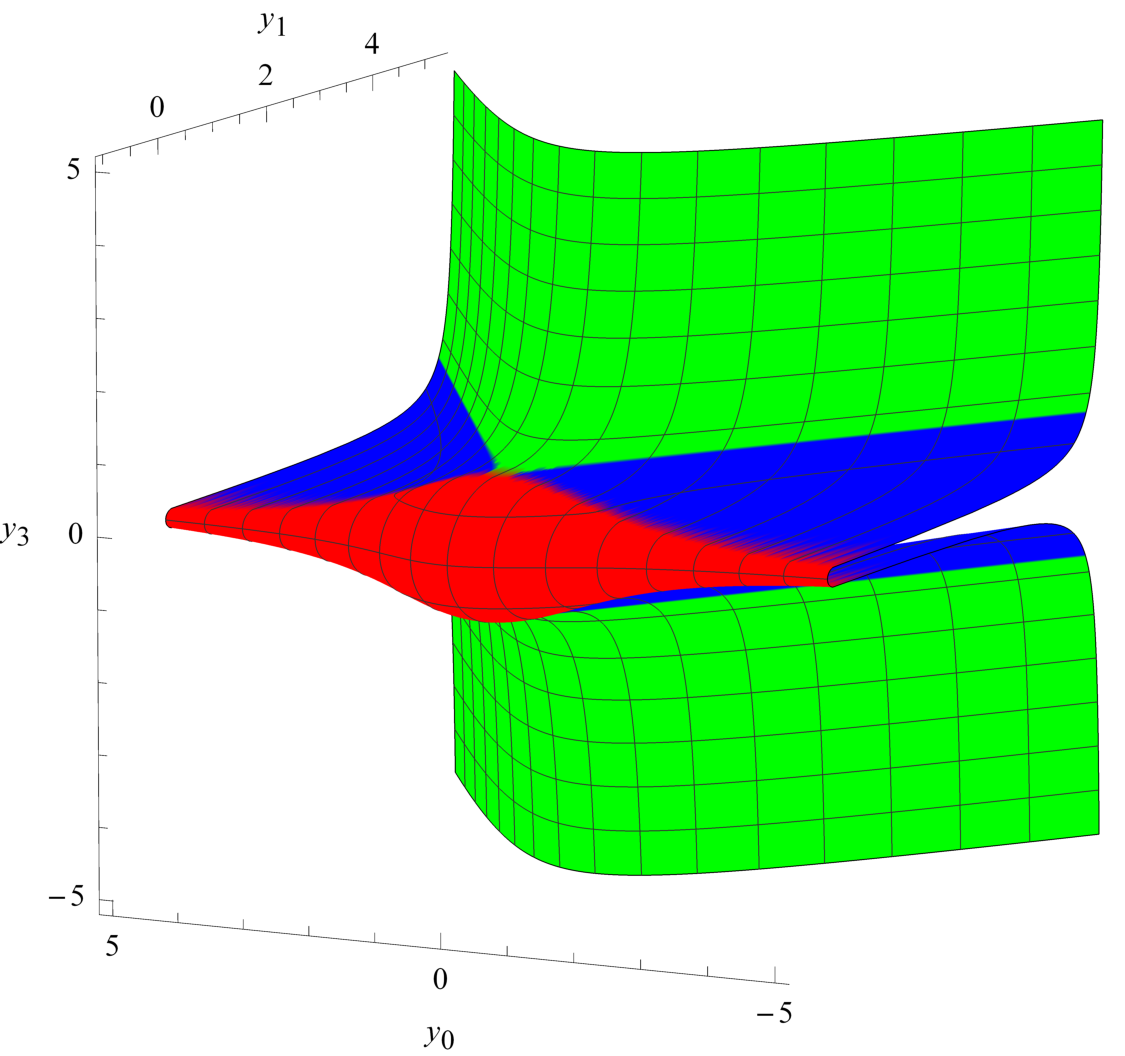
\includegraphics[width=0.55\linewidth]{col_emb42-c2.pdf}
\caption{\label{pic_emb}
Проекция двумерного подмногообразия $\theta,\varphi=const$ вложения \eqref{sp16},\eqref{sp18} на подпространство $y^0,y^1,y^3$.
%The section $y^4 = y^5 = 0$ in the coordinates $ y^0 $, $ y^1 $ and $ y^3 $.
}
\end{figure}
Красным показана область область пыли,
зеленым и синим -- область вне пылевого шара над и под горизонтом, соответственно.
Сингулярностям в прошлом и в будущем соответствуют пределы $y^0\to\pm\infty$.

Построенное вложение \eqref{sp16},\eqref{sp18}, как и полученное в разделе~3 вложение \eqref{sp10},
имеет гладкость, соответствующую физической постановке задачи (скачку плотности материи).
Его преимуществом является наличие только одного времениподобного направления в объемлющем пространстве,
однако с физической точки зрения оно описывает физически менее интересную чем \eqref{sp10} ситуацию
движения материи под вечно существующим горизонтом, в то время как \eqref{sp10} описывает динамическое формирование горизонта.


{\bf Acknowledgements.}
The work of A. K. is supported by a grant from the Russian Foundation for Basic Research (Project No. 18-31-00169).

\bibliographystyle{my3beznazv}
\bibliography{paston-grav-e}
\end{document}


